\documentclass[10pt]{beamer}
\usefonttheme{professionalfonts,serif}
\def\newblock{\hskip .11em plus .33em minus .07em}
\usepackage[numbers,sort]{natbib}
\renewcommand{\rmdefault}{psbx}
\usepackage[utf8]{inputenc}
\usepackage[T1]{fontenc}
\usepackage{textcomp}
\usepackage{eulervm}

\usetheme{default}           % tips from David Blei
\useinnertheme{circles}
\useoutertheme{infolines}
\setbeamertemplate{headline}{}
\setbeamertemplate{navigation symbols}{}
\setbeamerfont{itemize/enumerate subbody}{size=\normalsize}
\setbeamerfont{itemize/enumerate subsubbody}{size=\normalsize}
\usecolortheme{seahorse}
\setbeamersize{text margin left=2mm,text margin right=2mm}

\graphicspath{{../../figures/}}

\definecolor{mypine}{rgb}{0.05,0.45,0.05}
\definecolor{mycyan}{rgb}{0.0,0.9,0.9}
\newcommand{\Red}{\textcolor{red}}
\newcommand{\Blue}{\textcolor{blue}}
\newcommand{\Green}{\textcolor{mypine}}
\newcommand{\PineGreen}{\textcolor{mypine}}
\newcommand{\Magenta}{\textcolor{magenta}}
\newcommand{\Cyan}{\textcolor{mycyan}}

\newcommand{\N}{\mathcal{N}}
\newcommand{\R}{\mathbb{R}}
\newcommand{\T}{{\scriptsize^{\top}}}
\newcommand{\D}{\mathcal{D}}
\newcommand{\F}{\mathcal{F}}
\newcommand{\E}{\mathbb{E}}
\newcommand{\V}{\mathbb{V}}
\newcommand{\M}{\mathcal{M}}
\newcommand{\KL}{\mathcal{KL}}
\newcommand{\cut}[1]{}
\newcommand{\trace}{\operatorname{trace}}

\newcommand{\bmu}{{\boldsymbol{\mu}}}
\newcommand{\btheta}{\boldsymbol{\theta}}
\newcommand{\bepsilon}{\boldsymbol{\epsilon}}
\newcommand{\balpha}{\boldsymbol{\alpha}}
\newcommand{\bbeta}{\boldsymbol{\beta}}
\newcommand{\bphi}{\boldsymbol{\phi}}
\newcommand{\bPhi}{\boldsymbol{\Phi}}
\newcommand{\bSigma}{\boldsymbol{\Sigma}}
\newcommand{\bpi}{\boldsymbol{\pi}}
\newcommand{\blambda}{\boldsymbol{\lambda}}

\newcommand{\argmax}{\operatorname{argmax}}
\newcommand{\argmin}{\operatorname{argmin}}
\newcommand{\ci}{{\bot\negthickspace\negthickspace\bot}} % conditional indep.
\newcommand{\neigh}{\operatorname{ne}}
\newcommand{\vectr}[2]{  \left[ \!\!\begin{array}{c} #1 \\
      #2 \end{array} \!\!\right]}
\newcommand{\deff}{\stackrel{\mathrm{def}}{=}}
\newcommand{\deldel}[2]{\frac{\partial #1}{\partial #2}}

\newcommand{\maketilde}{\raisebox{0.4ex}{\tiny $\sim$}}
\newcommand{\bfa}{\mathbf a}
\newcommand{\bfb}{\mathbf b}
\newcommand{\bfe}{\mathbf e}
\newcommand{\bff}{\mathbf f}
\newcommand{\bfk}{\mathbf k}
\newcommand{\bfm}{\mathbf m}
\newcommand{\bfn}{\mathbf n}
\newcommand{\bfp}{\mathbf{p}}
\newcommand{\bfs}{\mathbf s}
\newcommand{\bfu}{\mathbf u}
\newcommand{\bfx}{\mathbf x}
\newcommand{\bfy}{\mathbf y}
\newcommand{\bft}{\mathbf t}
\newcommand{\bfv}{\mathbf v}
\newcommand{\bfw}{\mathbf w}
\newcommand{\bfA}{\mathbf A}
\newcommand{\bfI}{\mathbf I}
\newcommand{\bfK}{\mathbf K}


\title{Gaussian Process}
\author{Carl Edward Rasmussen}
\date{October 10th, 2016}

\begin{document}

\begin{frame}
\titlepage
\end{frame}

\begin{frame}
\frametitle{Key concepts}
\begin{itemize}
\item generalize: scalar Gaussian, multivariate Gaussian, Gaussian process
\item \Blue{Key insight}: functions are like infinitely long vectors
\item \Blue{Surprise}: Gaussian processes are practical, because of
\begin{itemize}
\item the marginalization property
\end{itemize}
\item generating from Gaussians
\begin{itemize}
\item joint generation
\item sequential generation
\end{itemize}
\end{itemize}
\end{frame}

\begin{frame}
\frametitle{The Gaussian Distribution}
\begin{center}
\begin{tabular}{cc}
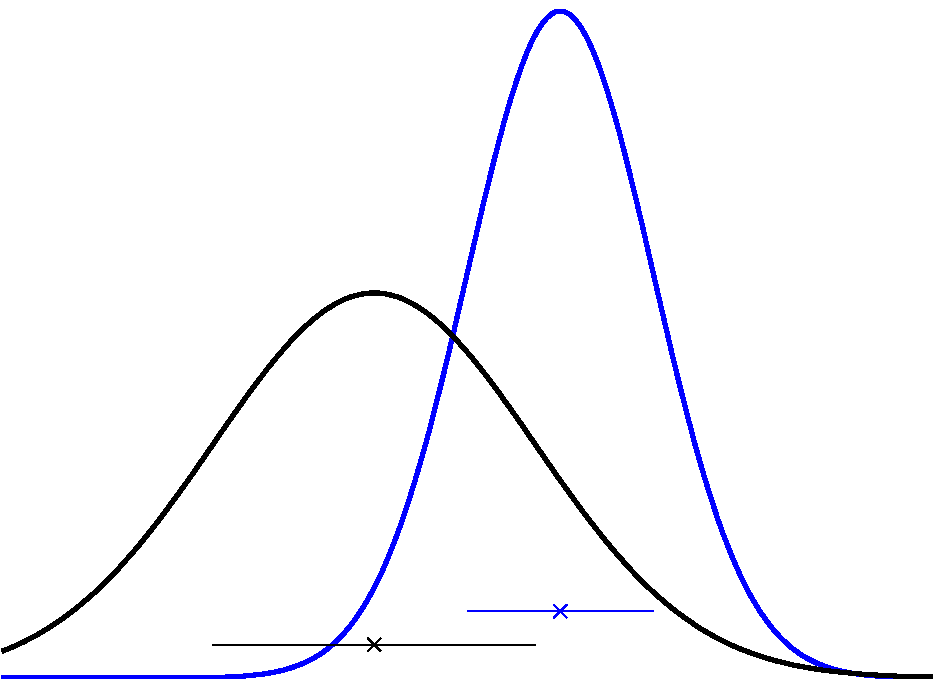
\includegraphics[width=0.4\textwidth]{gauss00} &
{
\includegraphics[width=0.4\textwidth]{gauss01}}
\end{tabular}
\end{center}
The univariate Gaussian distribution is given by
\[
p(x|\mu,\sigma^2) \;=\; (2 \pi \sigma^2 )^{-1/2} \exp \big( - \frac{1}{2
  \sigma^2} (x-\mu)^2 \big)
\]
The multivariate Gaussian distribution for $D$-dimensional vectors is given by
\[
p(\bfx|\mu,\Sigma)\;=\;{\cal N}(\mu,\Sigma)\;=\;(2\pi)^{-D/2}|\Sigma|^{-1/2}
\exp\big(-\tfrac{1}{2}(\bfx-\mu)^\top\Sigma^{-1}(\bfx-\mu)\big)
\]
where $\mu$ is the mean vector and $\Sigma$ the covariance matrix.
\end{frame}


\begin{frame}
\frametitle{Conditionals and Marginals of a Gaussian, pictorial}
\begin{center}
\begin{tabular}{cc}
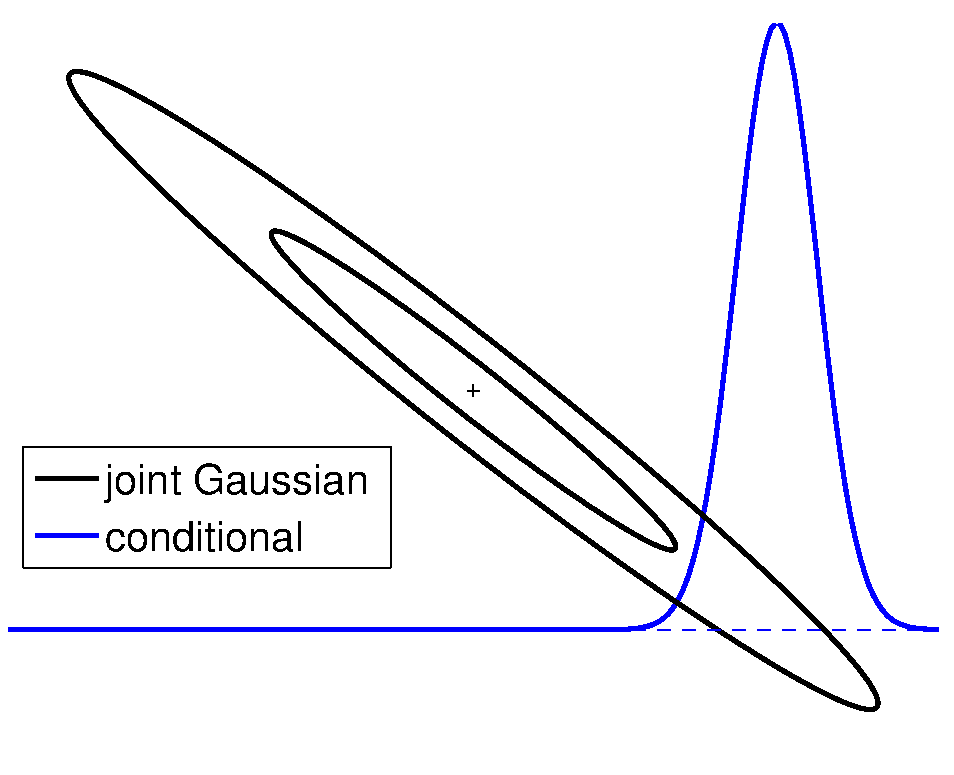
\includegraphics[width=0.45\textwidth]{gauss02} &
{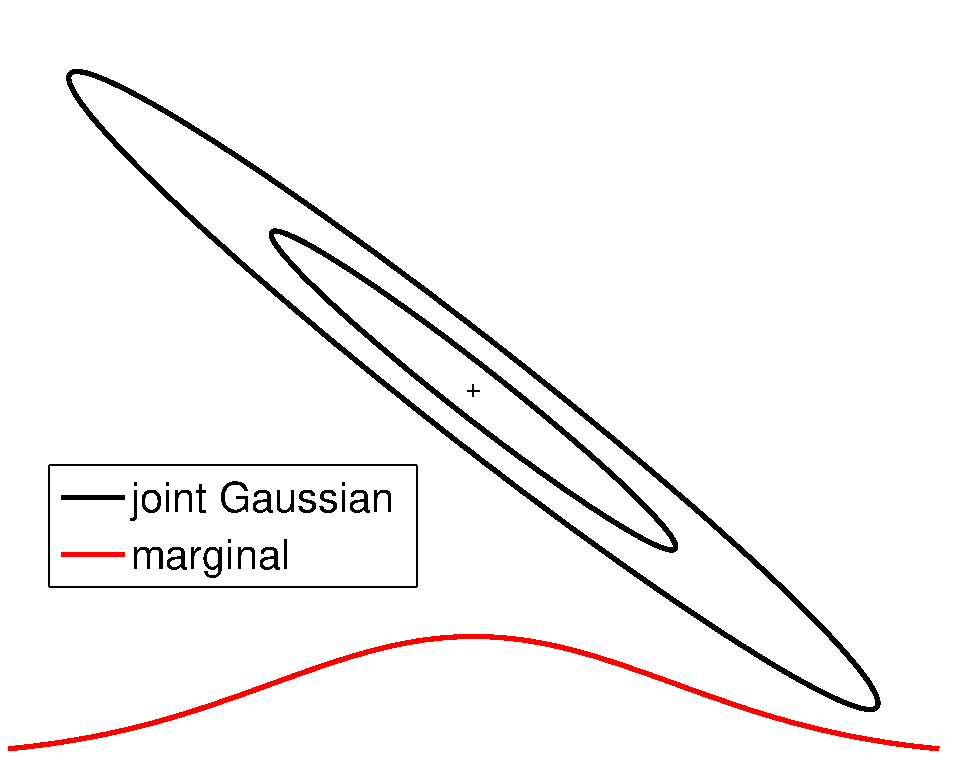
\includegraphics[width=0.45\textwidth]{gauss03}}
\end{tabular}
\end{center}

Both the \Blue{conditionals $p(x|y)$} and the \Red{marginals $p(x)$}
of a joint Gaussian $p(x,y)$ are again Gaussian.
\end{frame}


\begin{frame}
\frametitle{Conditionals and Marginals of a Gaussian, algebra}

If ${\bf x}$ and ${\bf y}$ are jointly Gaussian
\[
p(\bfx,\bfy)\;=\;p\big(\Big[\!\begin{array}{c}\bfx\\ \bfy\end{array}
\!\Big]\big)\;=\;{\cal N}\big(\Big[\!\begin{array}{c}{\bf a} \\ {\bf b}\end{array}\!\Big],
\;\Big[\!\begin{array}{cc}A & B \\ B^\top & C\end{array}\!\Big]\big),
\]

we get the marginal distribution of ${\bf x}$, $p(\bfx)$ by
\[
p(\bfx,\bfy)\;=\;{\cal N}\big(\Big[\!\begin{array}{c}{\bf a} \\ {\bf b}
\end{array}\!\Big],
\;\Big[\!\begin{array}{cc}A & B \\ B^\top & C\end{array}\!\Big]\big)
\;\;\Longrightarrow\;\;p(\bfx)\;=\;{\cal N}({\bf a},\;A),
\]

and the conditional distribution of ${\bf x}$ given ${\bf y}$ by
\[
p(\bfx,\bfy)={\cal N}\big(\Big[\!\begin{array}{c}{\bf a} \\ {\bf b}
\end{array}\!\Big],
\;\Big[\!\begin{array}{cc}A & B \\ B^\top & C\end{array}\!\Big]\big)
\;\Longrightarrow\;p(\bfx|\bfy)={\cal N}({\bf a}+BC^{-1}(\bfy-\bfb),\;
A-BC^{-1}B^\top),
\]

where ${\bf x}$ and ${\bf y}$ can be scalars or vectors.
\end{frame}


\begin{frame}
\frametitle{What is a Gaussian Process?}

A \emph{Gaussian process} is a generalization of a multivariate Gaussian
distribution to \Red{infinitely many variables}.

Informally: infinitely long vector $\simeq$ function

\begin{quote}
{\bf Definition}: a \emph{Gaussian process} is a collection of random
variables, any finite number of which have (consistent) Gaussian
distributions.\hfill$\Box$
\end{quote}

A Gaussian \Blue{distribution} is fully specified by a mean vector, $\mu$, and
covariance matrix $\Sigma$:
\[
\bff\;=\;(f_1,\ldots,f_N)^\top\;\sim\;{\cal N}(\mu,\Sigma),
\text{\ \ \ indexes\ } n=1,\ldots,N
\]
A Gaussian \Blue{process} is fully specified by a mean function $m(x)$ and
covariance function $k(x,x')$:
\[
f\;\sim\;{\cal GP}(m,k), \text{\ \ \ indexes:\ }x \in
{\cal X}
\]
here $f$ and $m$ are functions on ${\cal X}$, and $k$ is a function on
${\cal X} \times {\cal X}$
\end{frame}


\begin{frame}
\frametitle{The marginalization property}

Thinking of a GP as a Gaussian distribution with an infinitely long mean vector
and an infinite by infinite covariance matrix may seem impractical\ldots

\ldots luckily we are saved by the \emph{marginalization property}:

Recall:
\[
p(\bfx)\;=\;\int p(\bfx,\bfy)d\bfy.
\]

For Gaussians:
\[
p(\bfx,\bfy)\;=\;{\cal N}\big(\Big[\!\begin{array}{c}{\bf a} \\ {\bf b}
\end{array}\!\Big],
\;\Big[\!\begin{array}{cc}A & B \\ B^\top & C\end{array}\!\Big]\big)
\;\;\Longrightarrow\;\;p(\bfx)\;=\;{\cal N}({\bf a},\;A)
\]
\end{frame}


\begin{frame}
\frametitle{Random functions from a Gaussian Process}

Example one dimensional Gaussian process:
\[
p(f)\;\sim\;{\cal GP}\big(m,\;k\big),
\text{\ \ where\ \ }m(x) = 0,\text{\ \ and\ \ }k(x,x') = \exp(-\tfrac{1}{2}(x-x')^2).
\]
%
To get an indication of what this distribution over functions looks like, focus
on a finite subset of function values
$\bff=(f(x_1),f(x_2),\ldots,f(x_N))^\top$, for which
\[
\bff\;\sim\;{\cal N}(0, \Sigma),\text{\ \ where\ \ }\Sigma_{ij}=k(x_i,x_j).
\]
%
Then plot the coordinates of $f$ as a function of the corresponding $x$ values.
\centerline{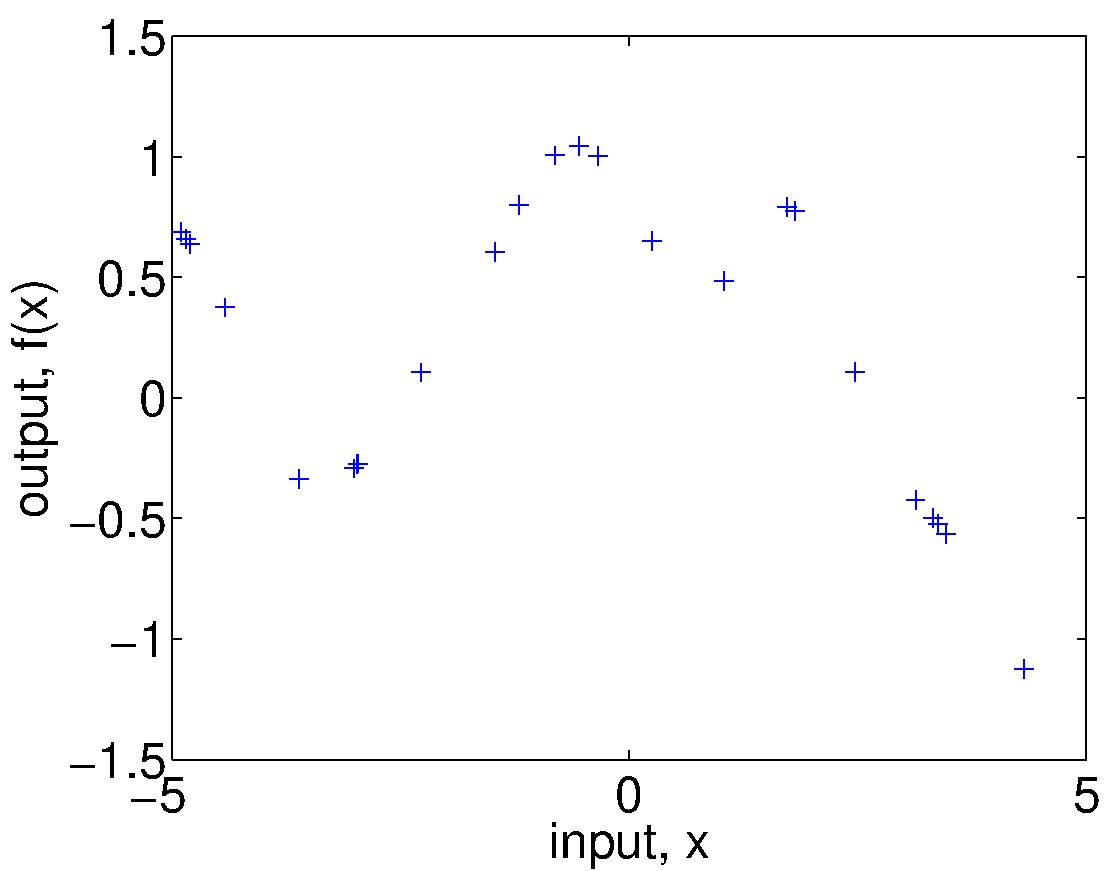
\includegraphics[width=0.5\textwidth]{prior1}}
\end{frame}


\begin{frame}[fragile]
\frametitle{Joint Generation}

To generate a random sample from a D dimensional joint Gaussian with
covariance matrix $K$ and mean vector ${\bf m}$: (in octave or matlab)

\begin{verbatim}
  z = randn(D,1);
  y = chol(K)'*z + m;
\end{verbatim}

where \texttt{chol} is the Cholesky factor $R$ such that $R^\top R=K$.

Thus, the covariance of $\bfy$ is:
\[
\mathbb{E}[(\bfy-{\bf m})(\bfy-{\bf m})^\top]\;=\;\mathbb{E}[R^\top{\bf z}
{\bf z}^\top R]\;=\;R^\top\mathbb{E}[{\bf z}{\bf z}^\top]R\;=\;R^\top IR\;=\;K.
\]
\end{frame}


\begin{frame}
\frametitle{Sequential Generation}

Factorize the joint distribution
\[
p(f_1,\ldots,f_N|x_1,\ldots x_N)\;=\;\prod_{n=1}^N
p(f_n|f_{n-1},\ldots,f_1,x_n,\ldots,x_1),
\]
and generate function values sequentially. For Gaussians:
\begin{align*}
p(f_n,f_{<n})&\;=\;{\cal N}\big(\Big[\!\!\begin{array}{c}{\bf a} \\ {\bf b}
\end{array}\!\!\Big],\Big[\!\!\begin{array}{cc}A\!\!&\!\!B \\ B^\top\!\!&\!\!C\end{array}\!\!\Big]\big)
\;\Longrightarrow\\
p(f_n|f_{<n})&\;=\;{\cal N}({\bf a}+BC^{-1}(f_{<n}-\bfb),\; A-BC^{-1}B^\top).
\end{align*}
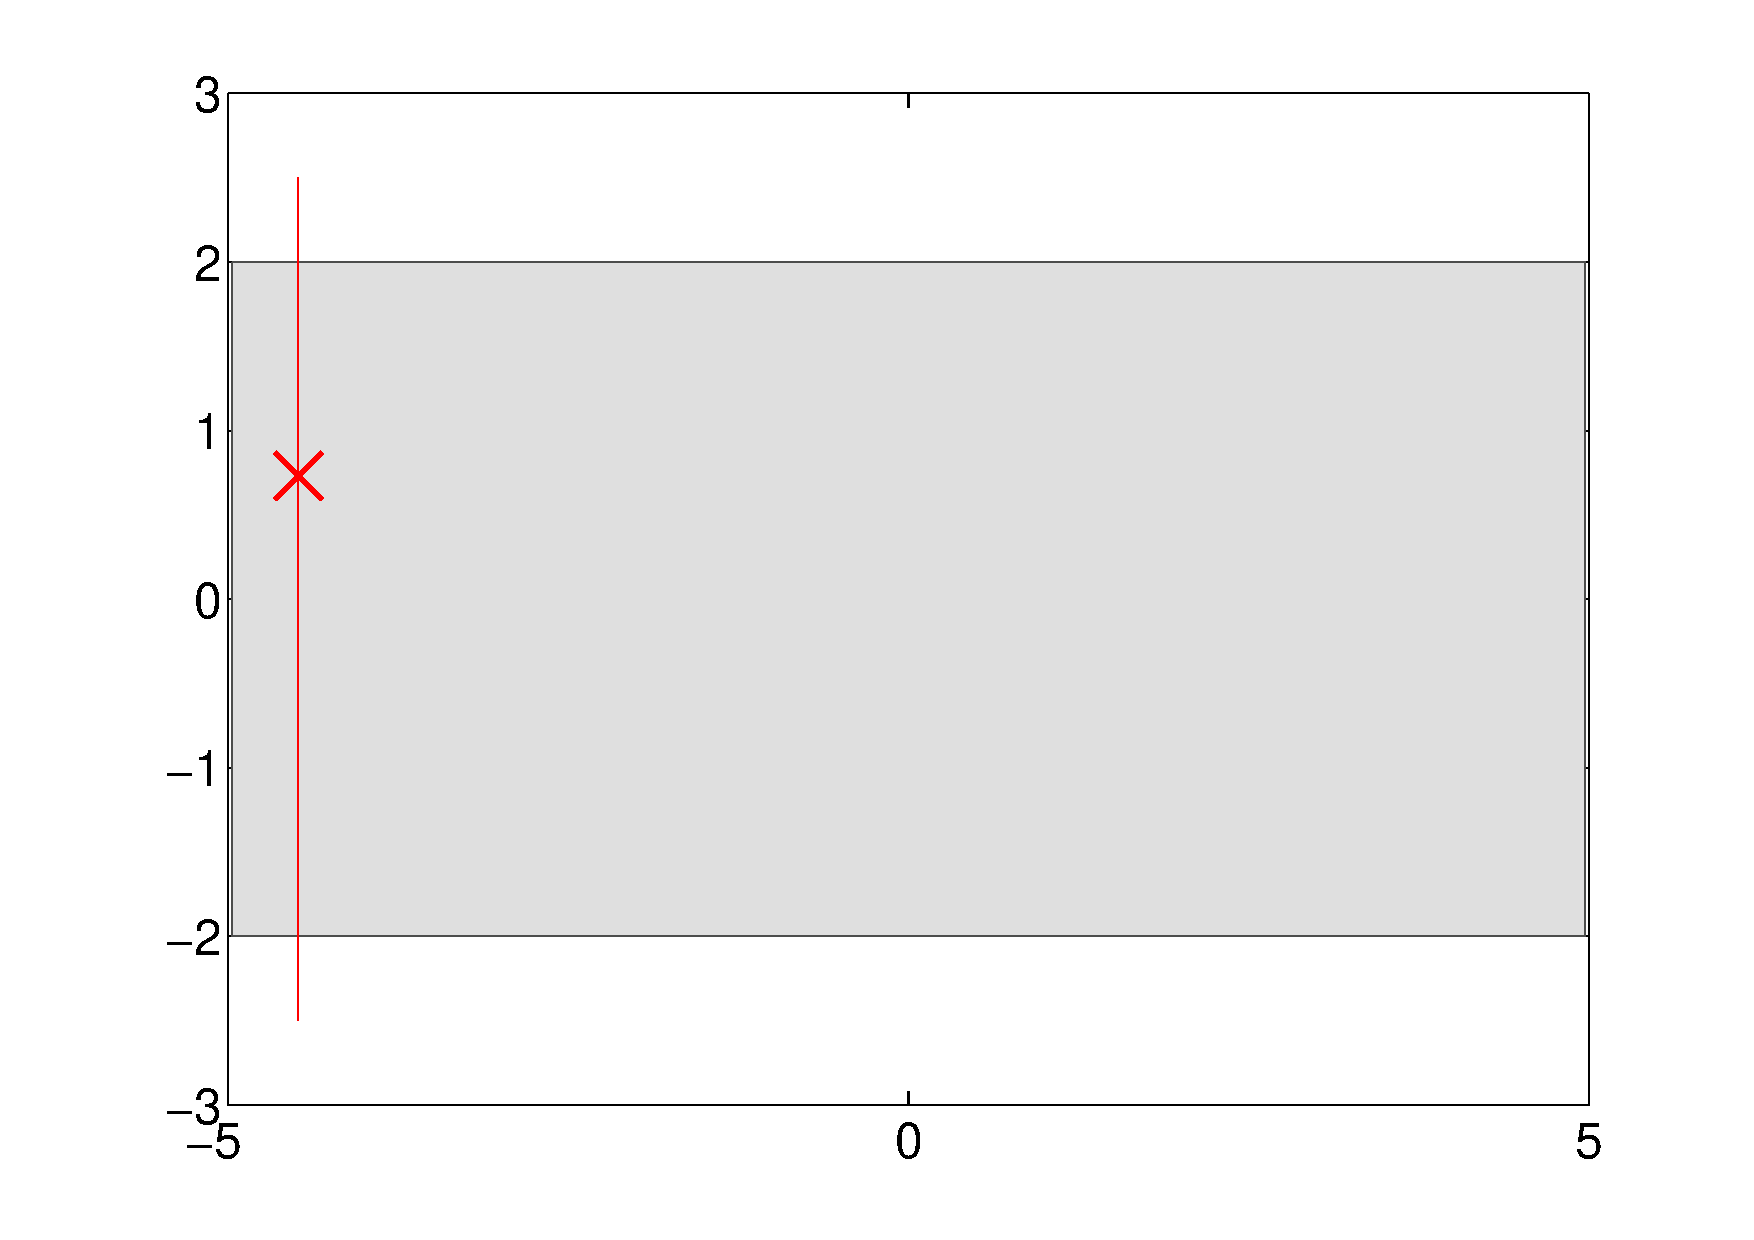
\includegraphics[width=0.33\textwidth]{seq_fullGP_M1.pdf}
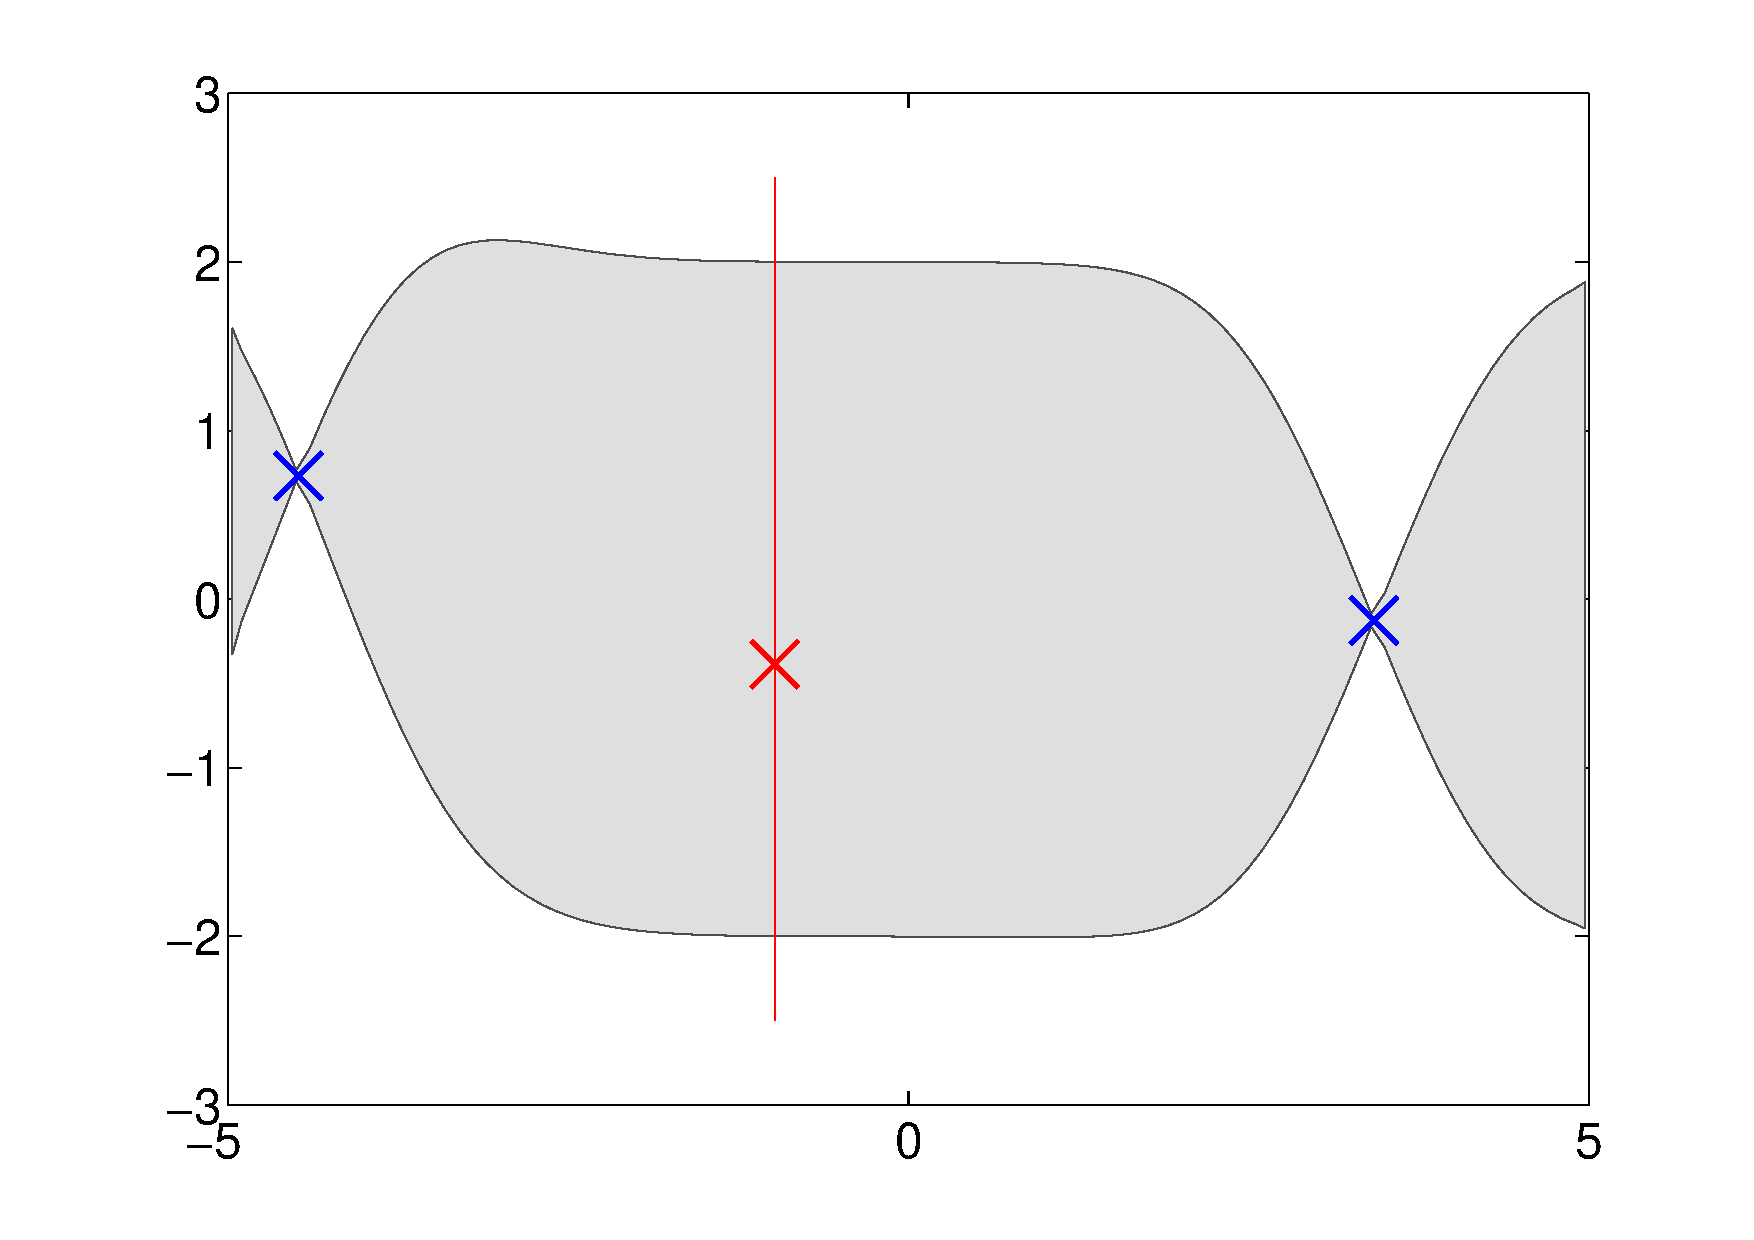
\includegraphics[width=0.33\textwidth]{seq_fullGP_M3.pdf}
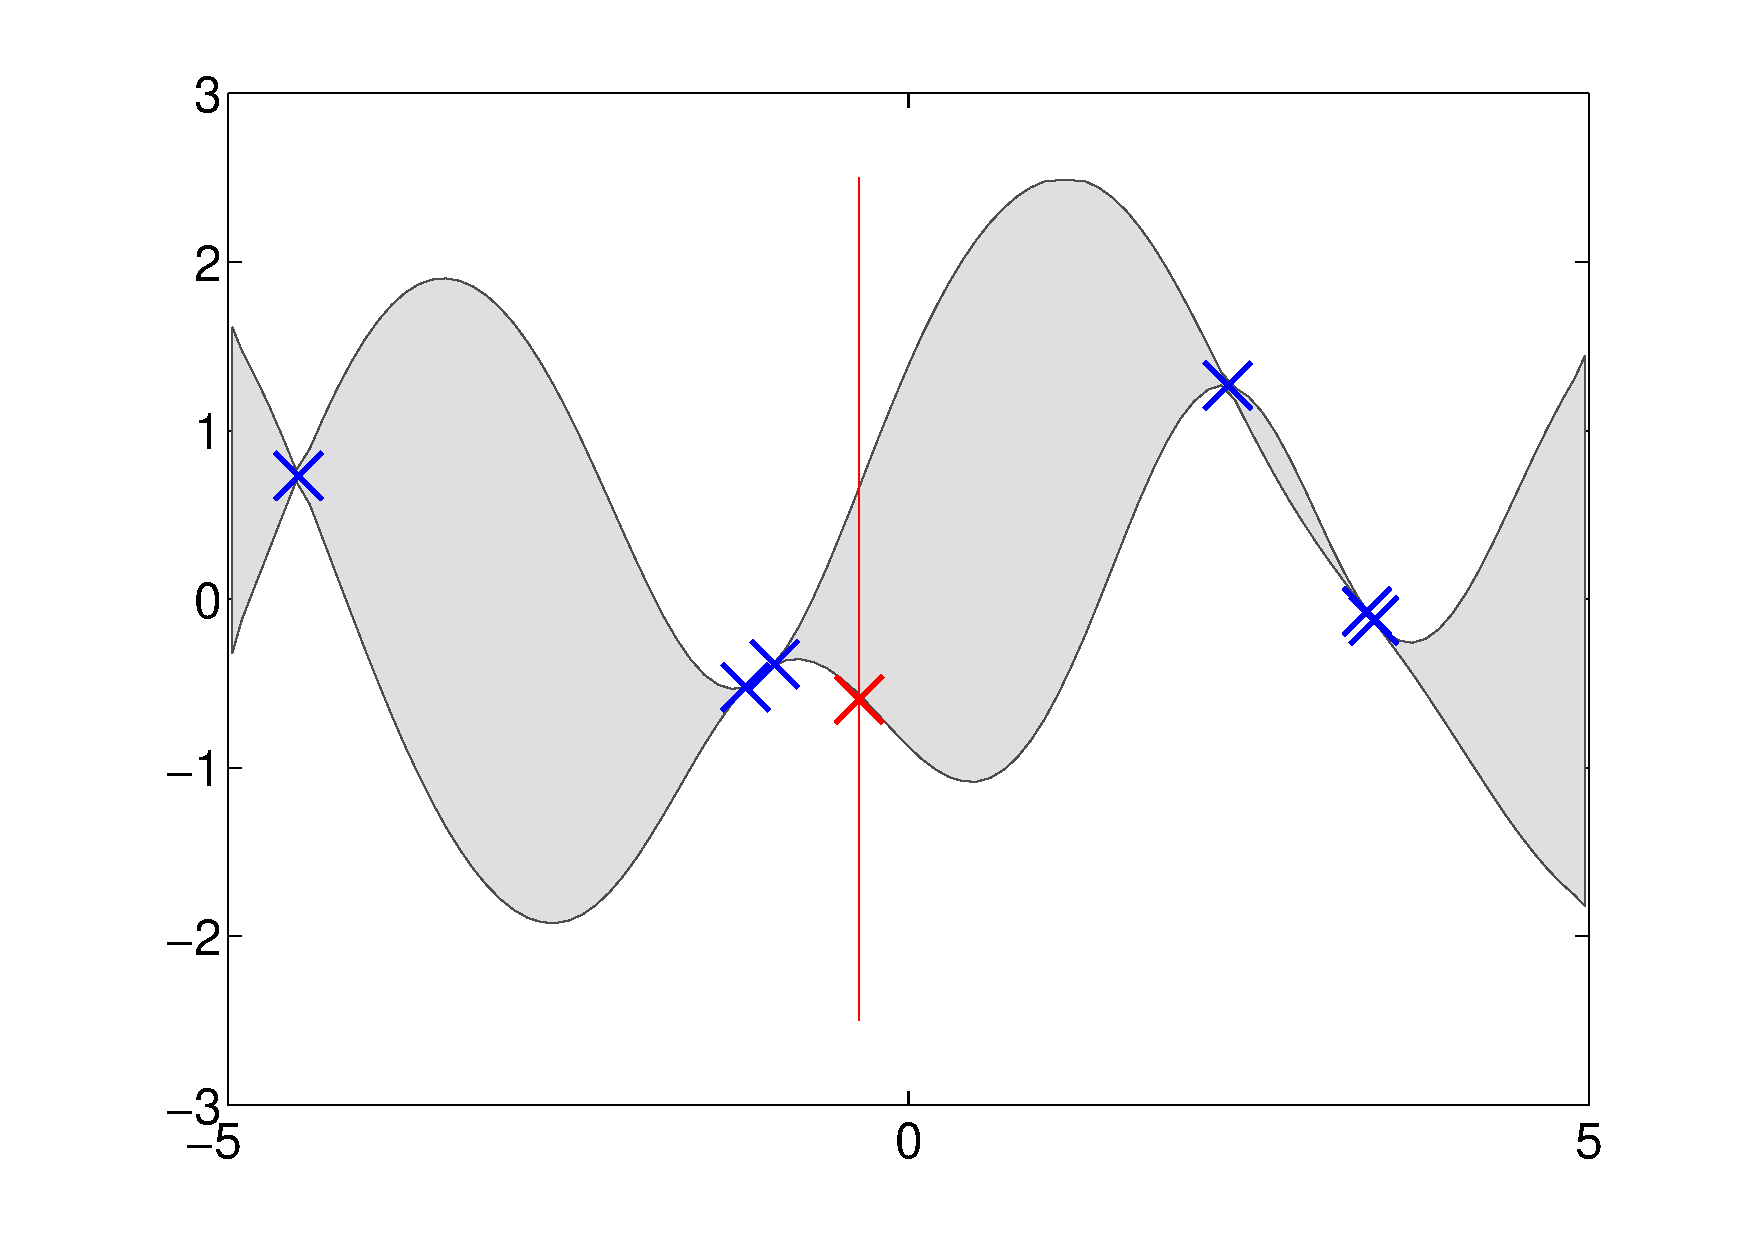
\includegraphics[width=0.33\textwidth]{seq_fullGP_M7.pdf}
\end{frame}


\begin{frame}
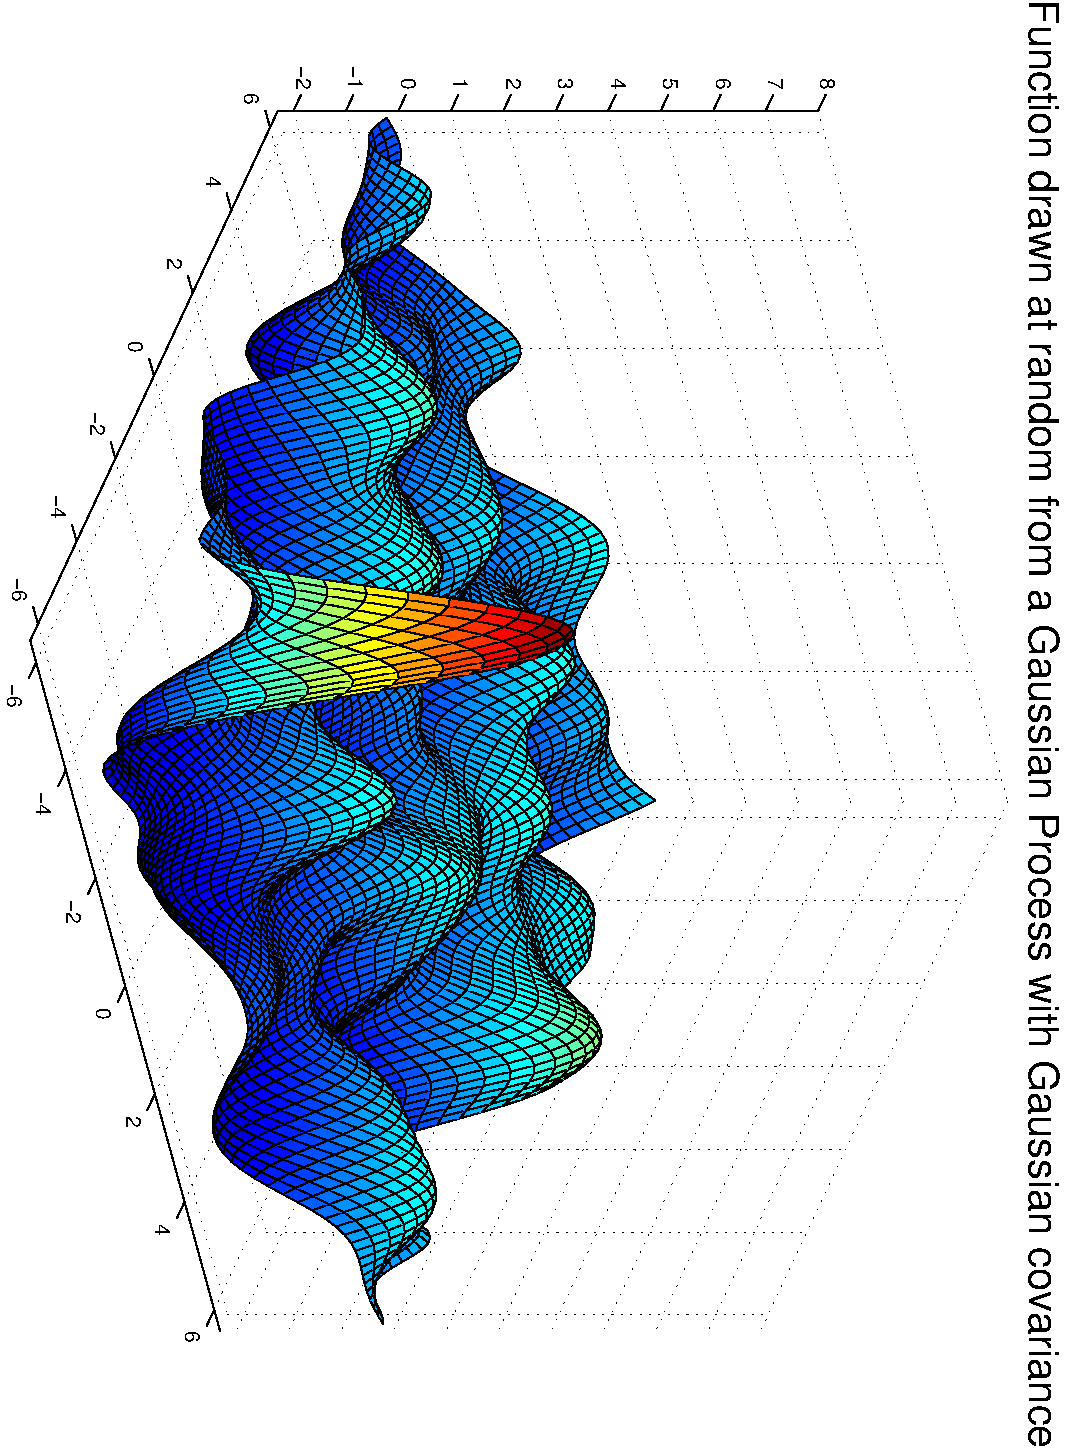
\includegraphics[height=\textwidth,angle=90]{gpprior}
\end{frame}
\end{document}
